% Sources: pretrain.py; utils/pretraining_trainer.py, pretraining_loss.py.
% Configuration: configs/pretraining.yaml. No decoder in this training path.
\documentclass[border=5pt]{standalone}
\usepackage[T1]{fontenc}
\usepackage{lmodern,amsmath,amssymb,tikz}
\usetikzlibrary{arrows.meta,calc}
\renewcommand{\familydefault}{\sfdefault}
\definecolor{edge}{HTML}{36424B}
\definecolor{global}{HTML}{E0EFEB}
\definecolor{local}{HTML}{E8E5F3}
\definecolor{encoder}{HTML}{E5EDF7}
\definecolor{loss}{HTML}{F8EDDA}
\begin{document}
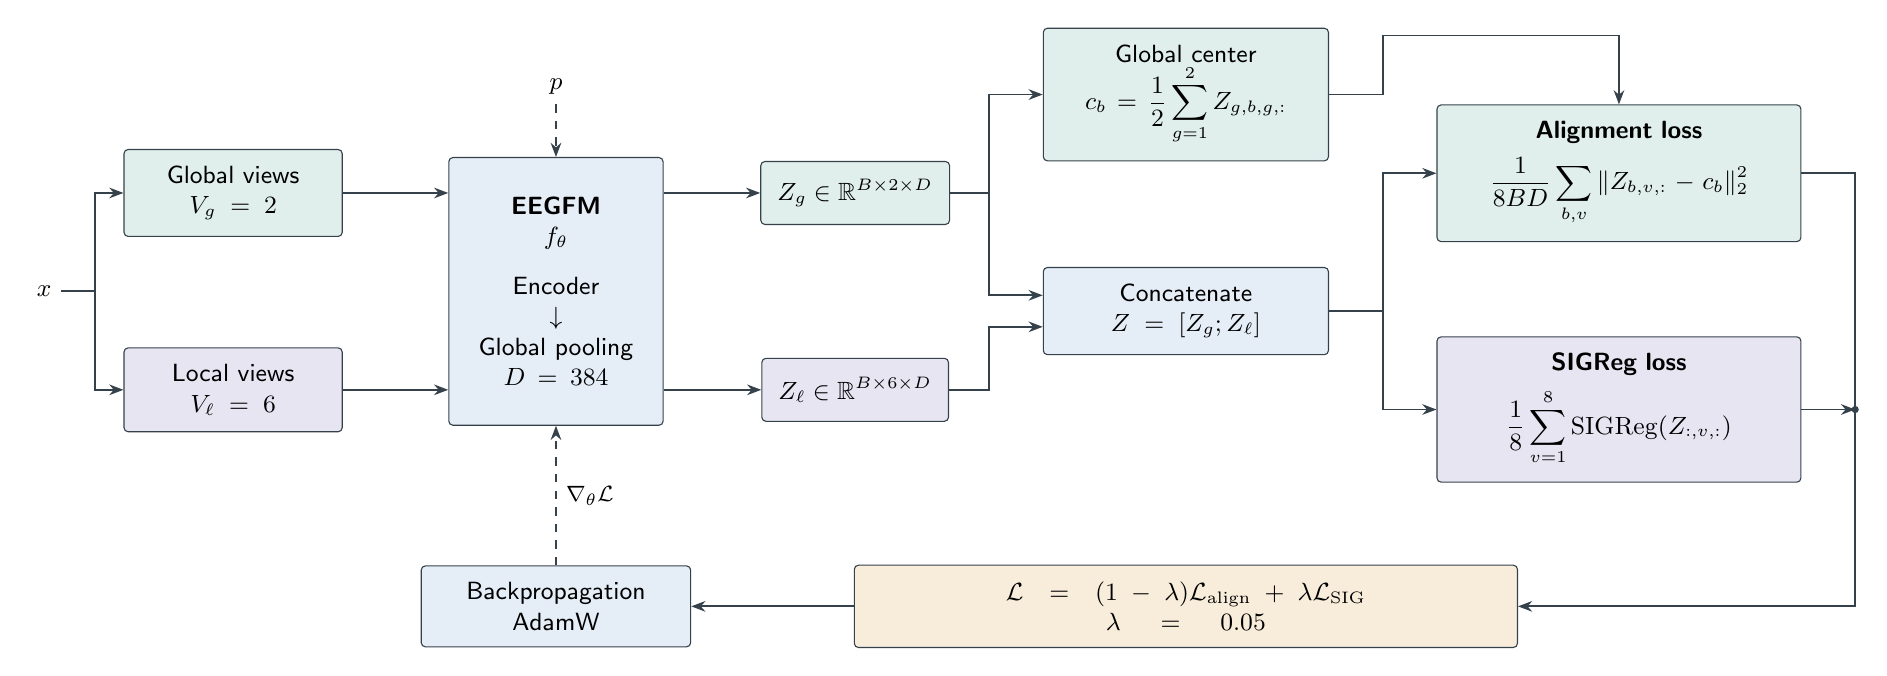
\begin{tikzpicture}[font=\small,x=1cm,y=1cm,>={Stealth[length=1.8mm]},
 block/.style={draw=edge,rounded corners=1.5pt,align=center,inner sep=6pt,minimum height=.8cm},
 flow/.style={->,draw=edge,line width=.65pt},
 label/.style={font=\footnotesize,align=center}]
\node (x) at (0,0) {$x$};
\node[block,fill=global,text width=2.35cm] (vg) at (2.4,1.25) {Global views\\$V_g=2$};
\node[block,fill=local,text width=2.35cm] (vl) at (2.4,-1.25) {Local views\\$V_\ell=6$};
\node[block,fill=encoder,text width=2.3cm,minimum height=3.4cm] (enc) at (6.5,0) {\textbf{EEGFM}\\$f_\theta$\\[7pt]Encoder\\$\downarrow$\\Global pooling\\$D=384$};
\node[block,fill=global] (zg) at (10.3,1.25) {$Z_g\in\mathbb{R}^{B\times2\times D}$};
\node[block,fill=local] (zl) at (10.3,-1.25) {$Z_\ell\in\mathbb{R}^{B\times6\times D}$};
\node[block,fill=global,text width=3.2cm] (center) at (14.5,2.5) {Global center\\$\displaystyle c_b=\frac{1}{2}\sum_{g=1}^{2}Z_{g,b,g,:}$};
\node[block,fill=encoder,text width=3.2cm] (all) at (14.5,-.25) {Concatenate\\$Z=[Z_g;Z_\ell]$};
\node[block,fill=global,text width=4.2cm] (align) at (20,1.5) {\textbf{Alignment loss}\\[4pt]$\displaystyle\frac{1}{8BD}\sum_{b,v}\|Z_{b,v,:}-c_b\|_2^2$};
\node[block,fill=local,text width=4.2cm] (sig) at (20,-1.5) {\textbf{SIGReg loss}\\[4pt]$\displaystyle\frac{1}{8}\sum_{v=1}^{8}\operatorname{SIGReg}(Z_{:,v,:})$};
\draw[flow] (x)--(.65,0)|-(vg); \draw[flow] (.65,0)|-(vl);
\draw[flow] (vg.east)--(enc.west|-vg); \draw[flow] (vl.east)--(enc.west|-vl);
\draw[flow] (enc.east|-zg)--(zg); \draw[flow] (enc.east|-zl)--(zl);
\draw[flow] (zg.east)--(12,1.25)|-(center);
\draw[flow] (12,1.25)--(12,-.05)--(all.west|-{(12,-.05)});
\draw[flow] (zl.east)--(12,-1.25)--(12,-.45)--(all.west|-{(12,-.45)});
\draw[flow] (center.east)--(17,2.5)--(17,3.25)--(20,3.25)--(align.north);
\draw[flow] (all.east)--(17,-.25)|-(align.west);
\draw[flow] (17,-.25)|-(sig.west);
\node[block,fill=loss,text width=8cm] (total) at (14.5,-4) {$\mathcal{L}= (1-\lambda)\mathcal{L}_{\rm align}+\lambda\mathcal{L}_{\rm SIG}$\\$\lambda=0.05$};
\node[block,fill=encoder,text width=3cm] (opt) at (6.5,-4) {Backpropagation\\AdamW};
\draw[flow] (align.east)--(23,1.5)--(23,-4)--(total.east);
\draw[flow] (sig.east)--(23,-1.5);
\fill[edge] (23,-1.5) circle (1.3pt);
\draw[flow] (total)--(opt);
\draw[flow,dashed] (opt.north)--node[right,label]{$\nabla_\theta\mathcal{L}$}(enc.south);
\node (p) at (6.5,2.6) {$p$};
\draw[flow,dashed] (p)--(enc.north);
\end{tikzpicture}
\end{document}
